\section{Resultados e Discussões} \label{pontosResultados}

Ao aplicar o método de geração de imagens HDR proposto por Sen~\etal~\cite{hdrMovimento} sobre as imagens da base de dados, notou-se que em algumas delas foram gerados artefatos antes não existentes. A Figura \ref{figResTonemap} mostra a versão \textit{tonemapped} das imagens HDR geradas.

\begin{figure}[H]
  \centering 
  \subfloat[Objeto visto de frente.]
  {
    \includegraphics[height=5cm]{toneMapping/PontosFrente}
    \label{figResTonemapA}
  }  
  \quad %espaco separador
  \subfloat[Objeto visto por baixo.]
  {
    \includegraphics[height=5cm]{toneMapping/PontosBaixo}
    \label{figResTonemapB}
  }
  \quad %espaco separador
  \subfloat[Objeto visto por cima.]
  {
    \includegraphics[height=5cm]{toneMapping/PontosCima}
    \label{figResTonemapC}
  }
  \quad %espaco separador
  \subfloat[Objeto visto pela direita.]
  {
    \includegraphics[height=5cm]{toneMapping/PontosDireita}
    \label{figResTonemapD}
  }
  \quad %espaco separador
  \subfloat[Objeto visto pela esquerda.]
  {
    \includegraphics[height=5cm]{toneMapping/PontosEsquerda}
    \label{figResTonemapE}
  }
  \caption{Imagens HDR \textit{tonemapped} da base de dados.}
  \label{figResTonemap}
\end{figure}

É visívels na Figuras \ref{figResTonemapA}, \ref{figResTonemapB}, e \ref{figResTonemapE}, apresença de distorções e no caso da Figura \ref{figResTonemapB} a presença de mais grades que o esperado. Provavelmente estes problemas foram gerados devido ao movimento existente entre as imagens LDR que geraram as respectivas imagens HDR.

Foi feito então a comparação da obtenção de nuvem de pontos utilizando imagens convencionais em relação às imagens \textit{tonemapped} obtidas. Ao gerar a nuvem de pontos utilizando o conjunto de imagens LDR mais bem expostas, citado na Seção \ref{pontosBaseImg}, foi obtido resultado melhor que ao utilizar as figuras HDR \ref{tonemapped}. A Tabela \ref{tabResultados} mostra a média de pontos de interesse que foram corretamente correspondidos entre as imagens, assim como o número de pontos 3D obtidos nas nuvens de pontos de cada abordagem. E a Figura \ref{figNuvemPontos} mostra as nuvens de pontos obtidas.

\begin{table}[H]
  \centering
  \caption{Resultados obtidos com a geração das nuvens de pontos.}
  \label{tabResultados}
  \begin{tabular}{l|l|l}
    \hline
               & Média de correspondência &  Número de pontos 3D \\
               & dos pontos de interesse  \\
               & por par de imagens       \\
    \hline
    Imagens LDR convencionais & 183,6 & 1262 \\
    \hline
    Imagens \textit{tonemapped} & 139,3 & 937 \\  
    \hline
  \end{tabular}
\end{table}

\begin{figure}[H]
  \centering 
  \subfloat[Obtida utilizando imagens LDR convencionais.]
  {
    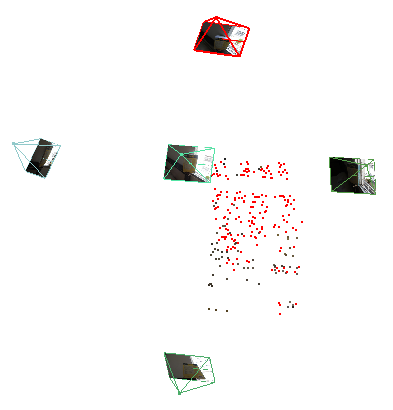
\includegraphics[height=5cm]{nuvemPontos/Convencional}
    \label{figNuvemPontosA}
  }  
  \quad %espaco separador
  \subfloat[Obtida utilizando as imagens \textit{tonemapped} geradas.]
  {
    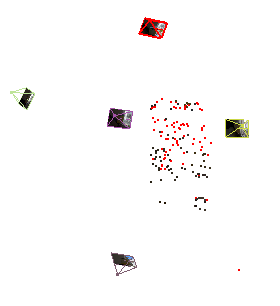
\includegraphics[height=5cm]{nuvemPontos/HDR}
    \label{figNuvemPontosB}
  }
  \caption{Nuvens de pontos obtidas utilizando o software VisualSFM.}
  \label{figNuvemPontos}
\end{figure}


Tendo em vista o resultado obtido com as imagens \textit{tonemapped}, optou-se por não dar continuidade ao processo proposto na Seção \ref{pontosProposta}. A justificativa disso é que por conta dos artefatos das imagens HDR geradas, ao realçá-las também haverá o realce dessas singularidades, levando a obtenção de pontos de interesse falsos e não úteis.